\documentclass{scrartcl}
\usepackage[utf8]{inputenc}
\usepackage{verbatim}
\usepackage{enumitem}
\usepackage{graphicx}
\usepackage[ngerman]{babel}
\usepackage{hyperref}
\usepackage{xcolor}
\hypersetup{
    colorlinks,
    linkcolor={blue!50!black},
    citecolor={blue!50!black},
    urlcolor={blue!80!black}
}

\usepackage[acronym,xindy,toc,nonumberlist]{glossaries} % nomain, if you define glossaries in a file, and you use \newglossaryentry{Client-Server-Architektur} 
	{
	name=Client-Server-Architektur,
	description={Konzept zur Verteilung von Aufgaben in Netzwerken. }
	}
	
	\newglossaryentry{Server} 
	{
	name=Server,
	description={Ein Server kommuniziert mit einem Client, um Aufgaben/Anfragen vom Client zu bearbeiten. }
	}
	
	\newglossaryentry{Client} 
	{
	name=Client,
	description={Ein Client kann Aufgaben/Anfragen an einen Server schicken. }
	}	
	
	\newglossaryentry{Tomcat} 
	{
	name=Tomcat,
	description={Tomcat führt in Java geschriebene Web-Anwendungen auf Servern aus. }
	}	
	
	\newglossaryentry{Android} 
	{
	name=Android,
	description={Android ist ein weitverbreitetes Betriebssystem für Smartphones, welches von Google entwickelt wurde.}
	}	
	
	\newglossaryentry{Gruppengrnder} 
	{
	name=Gruppengründer,
	description={Bezeichnet den Status des Mitglieds, das die Gruppe gegründet hat.}
	}
	
	\newglossaryentry{Mitglied}
	{
	name=Mitglied,
	description={Benutzer der einer Gruppe angehört.}
	}
	
	\newglossaryentry{Teilnehmer}
	{
	name=Teilnehmer,
	description={Ein Mitglied, das an einem Termin teilnimmt}
	}
\glossarystyle{altlist}
\makeglossaries
\usepackage[xindy]{imakeidx}

\makeindex
\loadglsentries[main]{INP-00-glossary}
\title{Android goApp - Pflichtenheft}
\author{Jörn Kussmaul, Katharina Riesterer, Julian Neubert,\\ Jonas Walter, Tobias Ohlsson, Eva-Maria Neumann}

\begin{document}
		
	

	\maketitle
	\newpage
	
	\tableofcontents
	\newpage
	%TODO Form
	%TODO Termin in Vergangenheit anlegen ?
	\section{Zielbestimmung}
	Das Ziel ist es eine Android Applikation für Gruppen sozial aktiver Menschen zu entwickeln. Diese ermöglicht es kurzfristig sich in einer Gruppe zu treffen. Hierfür können Termine erstellt werden, um das schnelle informieren der Gruppe zu gewährleisten.
	\subsection{Musskriterien}
	\begin{itemize}
		\item Anmeldung mit Google Services
		\item Ein Benutzer kann \gls{Mitglied} mehrerer Gruppen sein und kann Name, Mitglieder, Gründer und Termine einsehen
		\item Gruppenverwaltung
		\begin{itemize}
			\item Erstellen neuer Gruppen
			\item Suche bestehender Gruppen
			\item Gründer-Benutzer-Rollenstruktur
			\item Mitglieder in die Gruppe aufnehmen, aus der Gruppe entfernen
			\item Gruppe löschen
			\item Gruppenname ändern
		\end{itemize}
		\item Terminverwaltung
		\begin{itemize}
			\item Termine können mit Zeit, Ort, Name innerhalb einer Gruppe erstellt werden
			\item Benutzer können bei Terminen zu-/absagen
			\item Benutzer werden an ihren Termin erinnert
		\end{itemize}
		\item Ein Benutzer kann seinen eigenen Standort und den Gruppenmittelpunkt abrufen
	\end{itemize}
	\subsection{Wunschkriterien}
	\begin{itemize}
		\item \glqq{}Bin los\grqq{} und \glqq{}Bin da\grqq{} und \glqq{}Bin zu spät\grqq{}
		\begin{itemize}
			\item Benutzer können per Button signalisieren, ob sie bereits zum Treffpunkt unterwegs sind oder diesen sogar schon erreicht haben
			\item Nur Benutzer, die unterwegs sind, werden für den Gruppenmittelpunkt beachtet
			\item Benutzer, die den Treffpunkt erreicht haben, werden für die Berechnung des Gruppenmittelpunktes stärker beachtet
			\item Benutzer können der Gruppe mitteilen, dass sie zu spät sind
		\end{itemize}
		\item Der Gruppenmittelpunkt teilt sich bei Gruppenteilung
		\item Die Dauer eines Termins kann individuell festgelegt werden
		\item Individuelle Erinnerung pro Benutzer und pro Termin
		\item Erinnerung an Termine auch bei geschlossener App
		\item Termine können gelöscht, geändert und wiederholt werden
		\item Statistiken über die Teilnahme der Benutzer können eingesehen werden
		\item QR-Code oder Link zum Finden von Gruppen
		\item Sprachwahl
	\end{itemize}
	\subsection{Abgrenzungskriterien}
	\begin{itemize}
		\item Kein Chat
		\item Benutzer können nicht die Standorte andere Benutzer abfragen
		\item Der Gruppengründer kann keine neuen Mitglieder suchen
	\end{itemize}

	\newpage
	
	
	

	\section{Produkteinsatz}      
		Das Produkt soll das spontane Organisieren von Treffen unterstützen. Dazu soll es dem Benutzer möglich sein in einer Gruppe einen Termin zu erstellen, bzw. bei Terminen zu- oder abzusagen. \newline
		Kurz vor dem Termin wird dann der Gruppenmittelpunkt angezeigt, um das Finden der anderen Gruppenmitglieder zu erleichtern.

	\subsection{Anwendungsbereich}
	\begin{itemize}	        
		\item Spontane Terminvereinbarung von Gruppen
	\end{itemize}
	\subsection{Zielgruppe}
	\begin{itemize}	        
		\item Alle Studierende und Mitarbeiter am KIT
	\end{itemize}
	\subsection{Betriebsbedingung}
	\begin{itemize}	        
		\item App kann überall eingesetzt werden
		\item Für vollständigen Funktionsumfang benötigt man GPS und eine stabile Internetverbindung
	\end{itemize}
	
	\newpage
	
	
	\section{Produktumgebung}
	\begin{itemize}	        
		\item Eine \gls{Client-Server-Architektur}
		\item Der \gls{Client} ist ein Android-Gerät
		\item Die goApp läuft parallel mit anderen Apps auf einem Android-Gerät
	\end{itemize}
	\subsection{Software}
	\begin{itemize}	        
		\item \gls{Client}: \gls{Android} ab 4.4
		\item \gls{Server}: CentOS 6.8, \gls{Tomcat} 8, MySQL
	\end{itemize}	
	\subsection{Orgware}
	\begin{itemize}	        
		\item Internetverbindung
		\item Standortabfrage
	\end{itemize}
	\subsection{Produktschnittstelle}
	\begin{itemize}	        
		\item Google Maps
		\item Google Services
	\end{itemize}
	\subsection{Referenzgerät}
	\begin{itemize}
		\item Samsung Galaxy S4 (GT-I9505)
		\item \gls{Android} 5.0.1
	\end{itemize}
	\newpage
	
	
	\section{Funktionale Anforderungen}

	\renewcommand{\labelitemii}{$\bullet$}
	 In diesem Abschnitt sind die Aussagen über die zu erfüllenden Eigenschaften und zu erbringende Leistung unserer App vermerkt. Die mit \glqq WFAxx\grqq gekennzeichneten Anforderungen beziehen sich auf die Wunschkriterien der App.
	 
	\subsection{Kontoverwaltung}
	\begin{itemize}
		\item[FA10] Anmeldung eines Benutzers in der App über \gls{Google Services}
		\item[WFA15] Der Benutzer kann zwischen Sprachen wählen
		\item[FA20] Ersterfassung und Änderung des Benutzernamens
		
	\end{itemize}
	
	\subsection{Gruppenverwaltung}
	\begin{itemize}
		\item[FA30] Jeder Benutzer kann eine Gruppe erstellen
		\item[FA35] Ersterfassung und spätere Änderung des Gruppennamens durch den \gls{Gruppengrnder}
		\item[FA40] Gruppen können über den Gruppennamen gesucht werden
		\item[FA45] Benutzer können Beitrittsanfragen an eine Gruppe senden
		\item[FA50] Der \gls{Gruppengrnder} kann Beitrittsanfragen der Gruppe verwalten:
		\begin{itemize}
			\item Anfragen bestätigen, wodurch der Anfragende ein \gls{Mitglied} der Gruppe wird und die Anfrage gelöscht wird
		\end{itemize}
		\begin{itemize}
			\item Anfragen ablehnen, wodurch die Anfrage gelöscht wird
		\end{itemize}
		\begin{itemize}
			\item Anfragen ignorieren, wodurch die Anfrage bestehen und sichtbar bleibt
		\end{itemize}
		\item[FA60] Der \gls{Gruppengrnder} kann Mitglieder aus der Gruppe entfernen
		\item[FA70] Die Gruppe kann durch den \gls{Gruppengrnder} gelöscht werden
		\item[FA80] Mitglieder der Gruppen, ausgenommen des Gruppengründers, können die Gruppe verlassen
		\item[WFA85] Der \gls{Gruppengrnder} kann seinen Status als Gruppengründer an ein \gls{Mitglied} übergeben
		\item[FA90] Gruppenmitglieder können sich andere Gruppenmitglieder anzeigen lassen
		\item[WFA95] Gruppenmitglieder können die Teilnahmequoten anderer Gruppenmitglieder einsehen
		
	\end{itemize}
	
	\subsection{Terminverwaltung}
	\begin{itemize}
		\item[FA100] Jedes \gls{Mitglied} einer Gruppe kann einen Termin erstellen
		
		\begin{itemize}
			\item Ersterfassung von Terminnamen, Terminzeit (in der Zukunft) und Terminort
		\end{itemize}
		
		\begin{itemize}
			\item Visuelle Darstellung des gewählten Terminortes
		\end{itemize}
		\item[WFA105] Der Terminersteller kann den Terminnamen, Terminzeit und Terminort nachträglich ändern oder gegebenenfalls löschen
		\item[FA110] Der Gruppenmittelpunkt wird anhand der Standorte aller Teilnehmer berechnet		
		\item[FA120] Jeder Termin wird jedem Gruppenmitglied angezeigt
		\item[FA130] Jedes Gruppenmitglied kann bei einem Termin zu- oder absagen
		
	\end{itemize}
	
	\subsection{Terminablauf}
	\begin{itemize}
		\item[FA140] Jeder \gls{Teilnehmer} wird 30 Minuten vor Beginn des Termins benachrichtigt
		\item[WFA145] \gls{Teilnehmer} werden auch bei geschlossener App benachrichtigt
		\item[FA150] Jeder \gls{Teilnehmer} kann den Gruppenmittelpunkt ab 15 Minuten vor Beginn des Termins in einer Karte darstellen lassen
		\item[WFA155] Vom Gruppenmittelpunkt entfernte Teilgruppen  erhalten einen eigenen Standort 
		\item[WFA160] \gls{Teilnehmer} können in der App anderen Teilnehmern mitteilen,
		\begin{itemize}
			\item dass sie bereits unterwegs sind
			\item dass sie zu spät kommen
			\item dass sie schon am Terminort angekommen sind
		\end{itemize}
		\item[FA170] Der Termin löscht sich nach der Dauer des Termins (standardmäßig 60 Minuten)
		\item[WFA175] Die Dauer des Termins kann individuell festgelegt werden
	\end{itemize}
		
	
	\newpage
	
	
	\section{Produktdaten}
	
	\begin{itemize}
		\item [D10] Benutzerdaten:
		\newline Für jeden Benutzer werden die folgenden Daten gespeichert bzw. erfasst. Diese befinden sich auf dem Server, sowie lokal auf dem Client.
		\begin{itemize}
			\item Benutzername
			\newline Ein frei gewählter Name, der den anderen Benutzern der App angezeigt wird
			\item Standort
			\newline Der aktuelle Standort der Person, damit der Gruppenmittelpunkt berechnet werden kann. Dazu werden die aktuellen GPS Koordinaten des Geräts genutzt
			\item \gls{Google Services} Informationen
			\newline ID zur eindeutige Identifizierung der Benutzer
		\end{itemize}
		
		\item [WD15] Benutzerdaten:
\newline Die Statistiken werden auf dem Server und die Sprache auf dem Client gespeichert.
		\begin{itemize}
			\item Teilnahmen
			\newline Um Statistiken zu Erstellen, werden die Teilnahmen gespeichert
			\item Sprache
			\newline Die ausgewählte Sprache des Benutzers
			
		\end{itemize}
		
		
		\item [D20] Gruppendaten:
		\newline Eine Gruppe hat die folgenden Eigenschaften.
		Die Gruppendaten werden auf dem Server gespeichert. Zusätzlich werden von allen Gruppen in denen man Mitglied ist die ID und der Name lokal auf dem Client gespeichert.
		\begin{itemize}
			\item ID
			\newline ID-Nummer zur eindeutigen internen Identifikation
			\item Name
			\newline Angezeigter Name der Gruppe.
			\item Mitglieder
			\newline In einer Gruppe sind mehrere Benutzer
			\item Rechte
			\newline Die Mitglieder haben verschiedene Rechte. Der \gls{Gruppengrnder} hat mehr Rechte als die anderen Mitglieder und sein Name wird öffentlich in der Suche angezeigt.
			\item Termine
			\newline Eine Gruppe kann mehrere Termine haben
		\end{itemize}
		
		
		\item [WD25] Gruppendaten:
		\newline Die Links und QR-Codes werden auf dem Server gespeichert
		\begin{itemize}
			\item Link
			\newline Link zum Finden der Gruppe
			\item QR-Code
			\newline QR-Code zum Finden der Gruppe
		\end{itemize}
		
		\item [D30] Termindaten:
		\newline In der App gibt es mehrere aktive Termine gleichzeitig. Jeder Termin beinhaltet die folgenden Daten.
		Die Termine werden auf dem Server gespeichert, bis sie beendet sind. Zusätzlich dazu, sind zugesagte Termine auch lokal auf dem Client gespeichert.
		\begin{itemize}
			\item ID
			\newline ID-Nummer zur eindeutigen internen Identifikation
			\item Name
			\newline Der Name des Termins.
			\item Ziel
			\newline Das Ziel ist der Standort, wo das Treffen stattfinden soll
			\item \gls{Teilnehmer} Status
			\newline Status des Teilnehmers, ob er zu- oder abgesagt oder noch nicht reagiert hat
			\item Gruppe
			\newline Der Termin gehört zu einer bestimmten Gruppe
			\item Serverzeit
			\newline Datum und Uhrzeit des Treffens
		\end{itemize}
		
		\item [WD35] Termindaten:%TODO Mitteilungen glossar
Alle Termindaten werden auf dem Server gespeichert, außer der Erinnerung, diese wird auf dem Client gespeichert.
	 	\begin{itemize}
			\item Dauer
			\newline Die Dauer des Termins.
			\item Erinnerung
			\newline Festlegung des Zeitpunktes, wann der Benutzer an diesen Termin erinnert werden möchte.
			\item Wiederholung
			\newline Wenn der Termin wiederholt werden soll, wird hier die Frequenz der Wiederholung gespeichert.
			\item Mitteilung
			\newline Die Nachrichten durch diese sich Teilnehmer mitteilen können
		\end{itemize}
	\end{itemize}
	
	\newpage
	
	
	\section{Qualitative Anforderungen}
	Die Qualitativen Anforderungen beziehen sich auf unser Referenzgerät.
	\begin{itemize}
		\item[QA10] Die App soll auf jede Anfrage in durchschnittlich unter 5 Sekunden reagieren
		\item[QA20] Die App fährt in durchschnittlich unter 10 Sekunden hoch
		\item[QA30] Jede Funktion der App ist mit höchstens 5 Eingaben vom Startbildschirm der App zu erreichen
		\item[QA40] Bei 99\% aller Anwendungen werden Fehler abgefangen und führen nicht zum Absturz der App
		\item[QA50] Unterstützt bis zu 50 Benutzer pro Gruppe
		\item[QA60] Jeder Benutzer kann in bis zu 20 Gruppen \gls{Mitglied} sein
		\item[QA70] Der Server unterstützt das Anlegen von mindestens 30000 Benutzern
	\end{itemize}
	
	\newpage
	
	
	\section{Globale Testfälle}
%TODO Nummern der Funktionalen Anforderungen überprüfen
Die Tests werden auf dem Referenzgerät mit einer ausreichenden Internetverbindung und funktionierendem GPS ausgeführt. \newline
	Die folgenden Testfälle stellen sicher, dass die genannten Funktionalen Anforderungen erfüllt sind.
	
	\subsection{Kontoverwaltung}
	\begin{itemize} 
		\item[T10] deckt ab FA10 \newline
		Registrieren: Eine bisher nicht registrierte Person mit einem Google Account registriert sich mit diesem im System 				und wählt zusätzlich einen Benutzernamen. \newline
		Ergebnis: Der neue Benutzer mit seinem Google Account und Benutzername ist in der Datenbank.

		\item[T20] deckt ab FA20\newline
		Namensänderung: Ein Benutzer ändert seinen Benutzernamen. \newline
		Ergebnis: Der neue Benutzername des Benutzers ist in der Datenbank. 
	
	\subsection{Gruppenverwaltung}
	
		\item[T30] deckt ab FA30, FA35\newline
		 Ein beliebiger Benutzer erstellt eine neue Gruppe mit Namen. \newline
		Ergebnis: Eine neue Gruppe, mit eindeutiger Id, dem angegebenen Namen und dem Benutzer als Gründer, ist in der 			Datenbank.

		\item[T35] deckt ab FA35 \newline
		Der Gründer ändert den Gruppennamen.\newline
		Ergebnis: Auf dem Server ist bei der Gruppe der neue Name eingetragen. 

		\item[T40] deckt ab FA40, FA45  \newline
		Suchen der Gruppe nach Namen und eine Beitrittsanfrage an eine gefundene Gruppe stellen. \newline
		Ergebnis: Alle Gruppen-IDs der Gruppen, die die Suchanfrage im Namen enthalten. Anfrage in der Gruppe 		
		hinzugefügt.

		\item[T50] deckt ab FA50  \newline
		Der Gruppengründer bestätigt eine Anfrage. \newline
		Ergebnis: Der Benutzer der Anfrage ist \gls{Mitglied} der Gruppe und die Anfrage ist gelöscht.

		\item[T55] deckt ab FA50  \newline
		Der \gls{Gruppengrnder} lehnt eine Anfrage ab. \newline
		Ergebnis: Die Anfrage ist gelöscht.

		\item[T60] deckt ab FA60  \newline
		Der \gls{Gruppengrnder} entfernt ein Mitglied.  \newline
		Ergebnis: Der Benutzer ist nicht mehr Mitglied (Alle Assoziationen zwischen Gruppe und Benutzer sind getrennt).

		\item[T70] deckt ab FA70  \newline
		Der \gls{Gruppengrnder} löscht die Gruppe.  \newline
		Ergebnis: Alle Mitgliedern sind entfernt (FA60) und die Gruppe aus der Datenbank gelöscht.

		\item[T80] deckt ab FA80  \newline
		Ein Gruppenmitglied verlässt die Gruppe.  \newline
		Ergebnis: Der Benutzer ist nicht mehr \gls{Mitglied} (siehe T60).

	\subsection{Terminverwaltung}

		\item[T90] deckt ab FA100, FA110, FA120  \newline
		Ein beliebiges \gls{Mitglied} erstellt einen Termin mit Name, Ort, Zeitpunkt.  \newline
		Ergebnis: Es gibt einen Termin mit dem genannten Namen, Ort und Zeitpunkt in der Gruppe.
		
		\item [T100] deckt ab FA130  \newline
		Ein \gls{Mitglied} sagt ab.  \newline
		Ergebnis: Der Termin ist für das Mitglied gelöscht.

		\item[T105] deckt ab FA130  \newline
		Ein Mitglied sagt zu.  \newline
		Ergebnis: Das Mitglied ist \gls{Teilnehmer} des Termins und der Termin ist auf dem Gerät des Teilnehmers gespeichert.

	\subsection{Terminablauf}
	
		\item[T110] deckt ab FA140, FA150, FA170 \newline
		Automatischer Ablauf eines Termins. \newline
		Ergebnis: 30 Minuten vor dem Termin werden alle \gls{Teilnehmer} von dem Termin benachrichtigt.  \newline
			15 Minuten vor dem Terminzeitpunkt ist die Karte für alle Teilnehmer verfügbar.  \newline
			60 Minuten nach dem Terminzeitpunkt ist der Termin gelöscht (Keine Daten mehr zu diesem Termin, weder auf 					dem \gls{Client} noch auf dem \gls{Server}).

	\subsection{Standort}
%TODO Welche Funktionale Anforderung 
		\item[T120] deckt ab FA150 \newline
		Standort Übertragung der Clients an den \gls{Server}.  \newline
		Ergebnis: Der Standort aller \gls{Teilnehmer} ist auf dem Server gespeichert.

		\item[T130]  deckt ab FA150 \newline
		Der Server sendet den berechneten Gruppenmittelpunkt an den \gls{Teilnehmer}. \newline
		Ergebnis: Der Client hat den aktuellen Gruppenmittelpunkt.

	\end{itemize}	
	
	\newpage
	
	
	\section{Systemmodelle}
	
	\subsection{Anwendungsfälle}
	\subsubsection{Benutzer registrieren}
	\begin{description}
		\item \textbf{Titel:}
		\begin{description}
			\item Benutzer registrieren
		\end{description}
		\item \textbf{Kurzbeschreibung:}
		\begin{description}
			\item Der Benutzer registriert sich mit seinem Google Account.
		\end{description}
		\item \textbf{Aktoren:}
		\begin{description}
			\item Benutzer 
		\end{description}
		\item \textbf{Vorbedingungen:}
		\begin{description}
			\item Der Benutzer besitzt einen Google Account
			\item Mit diesem Google Account ist noch kein Konto verknüpft
		\end{description}
		\item \textbf{Ablauf:} \newline Für den Benutzer wird ein Konto auf der Datenbank erstellt und mit seinem Google Account verknüpft.
		\item \textbf{Ergebnis:} \newline Der Benutzer besitzt ein Konto und kann somit zu Gruppen hinzugefügt werden oder selber Gruppen erstellen.
	\end{description}
	
	\newpage
	
	\subsubsection{Gruppe erstellen}
	\begin{description}
		\item \textbf{Titel:}
		\begin{description}
			\item Gruppe erstellen
		\end{description}
		\item \textbf{Kurzbeschreibung:}
		\begin{description}
			\item Der Benutzer erstellt eine Gruppe.
		\end{description}
		\item \textbf{Aktoren:}
		\begin{description}
			\item Benutzer 
		\end{description}
		\item \textbf{Vorbedingungen:}
		\begin{description}
			\item Der Benutzer hat sich zuvor erfolgreich registriert.
		\end{description}
		\item \textbf{Ablauf:} \newline Es wird eine Gruppe erstellt, für die der erstellende Benutzer als Gruppengründer eingetragen wird. Der Benutzer muss einen Namen für seine Gruppe wählen. Damit erhält der Benutzer auch alle Rechte, die dem \gls{Gruppengrnder} zugestanden werden. 
		\item \textbf{Ergebnis:} \newline Der Benutzer ist \gls{Gruppengrnder} einer Gruppe und kann Benutzer zu dieser Gruppe hinzufügen oder Mitglieder aus der Gruppe entfernen. Des Weiteren hat er dieselben Rechte wie Mitglieder, er kann also auch Termine erstellen und an anderen Terminen innerhalb der Gruppe teilnehmen.
	\end{description}
	
	\newpage
	
	\subsubsection{Benutzer hinzufügen}
	\begin{description}
		\item \textbf{Titel:}
		\begin{description}
			\item Benutzer hinzufügen
		\end{description}
		\item \textbf{Kurzbeschreibung:}
		\begin{description}
			\item Der Gruppengründer fügt Benutzer hinzu.
		\end{description}
		\item \textbf{Aktoren:}
		\begin{description}
			\item \gls{Gruppengrnder}
			\item Benutzer
		\end{description}
		\item \textbf{Vorbedingungen:}
		\begin{description}
			\item Der Gruppengründer hat zuvor eine Gruppe gegründet und der Benutzer hat sich bereits registriert.
		\end{description}
		\item \textbf{Ablauf:} \newline Der Benutzer kann nach der Gruppe des Gruppengründers suchen und eine Beitrittsanfrage senden. Wurde die Anfrage gesendet kann der Gruppengründer sie einsehen und den Benutzer annehmen oder ablehnen. Hat der Gruppengründer den Benutzer angenommen, ist der Benutzer nun \gls{Mitglied} in der Gruppe und hat alle Rechte eines Mitglieds.
		\item \textbf{Ergebnis:} \newline Der Benutzer ist \gls{Mitglied} einer Gruppe und kann Termine erstellen oder an von anderen Personen innerhalb der Gruppe erstellten Terminen teilnehmen.
	\end{description}
	
	\newpage
	
	\subsubsection{Mitglied entfernen}
	\begin{description}
		\item \textbf{Titel:}
		\begin{description}
			\item Mitglied entfernen
		\end{description}
		\item \textbf{Kurzbeschreibung:}
		\begin{description}
			\item Der Gruppengründer entfernt ein Gruppenmitglied.
		\end{description}
		\item \textbf{Aktoren:}
		\begin{description}
			\item Gruppengründer
			\item Mitglied
		\end{description}
		\item \textbf{Vorbedingungen:}
		\begin{description}
			\item Der Gruppengründer hat zuvor eine Gruppe gegründet und das Mitglied wurde vom Gruppengründer in die Gruppe aufgenommen.
		\end{description}
		\item \textbf{Ablauf:} \newline Der Gruppengründer wählt in der Gruppenansicht das Mitglied aus, welches aus der Gruppe entfernt werden soll. Das Mitglied wird aus der Gruppe entfernt und wird zu einem normalen Nutzer der App.
		\item \textbf{Ergebnis:} \newline Das Mitglied gehört nicht mehr zu der Gruppe und kann somit keine Termine mehr einsehen oder ihnen beitreten. Termine an denen das Mitglied bereits teilnimmt, entfernen das Mitglied aus der Teilnehmerliste. Das Mitglied kann auch keine Informationen der Gruppe einsehen und wird als Nutzer betrachtet.
	\end{description}
	
	\newpage
	
	\subsubsection{Termin erstellen}
	\begin{description}
		\item \textbf{Titel:}
		\begin{description}
			\item Termin erstellen
		\end{description}
		\item \textbf{Kurzbeschreibung:}
		\begin{description}
			\item Ein Mitglied erstellt einen Termin.
		\end{description}
		\item \textbf{Aktoren:}
		\begin{description}
			\item \gls{Mitglied}
		\end{description}
		\item \textbf{Vorbedingungen:}
		\begin{description}
			\item Das Mitglied ist Mitglied einer Gruppe
		\end{description}
		\item \textbf{Ablauf:} \newline Das Mitglied erstellt innerhalb einer Gruppe einen Termin. Hierfür gibt er Namen, Uhrzeit und Ort für den Termin an. Das Mitglied, das den Termin erstellt nimmt automatisch an dem Termin teil. Der Termin ist an die Gruppe gebunden und alle anderen Mitglieder der Gruppe können die Informationen für diesen Termin einsehen und ihm beitreten.
		\item \textbf{Ergebnis:} \newline Das Mitglied hat einen an die Gruppe gebundenen, für alle Mitglieder sichtbaren, Termin erstellt. Mitglieder können an dem Termin als \gls{Teilnehmer} beitreten. Ein Teilnehmer wird eine halbe Stunde vor dem Termin benachrichtigt. Eine weitere viertel Stunde später kann er die Karte öffnen und den ungefähren Standort der anderen Teilnehmer dieses Termins einsehen.
	\end{description}
	
	\newpage
	
	\subsection{Anwendungsfalldiagramm}
	\begin{figure}[h]
		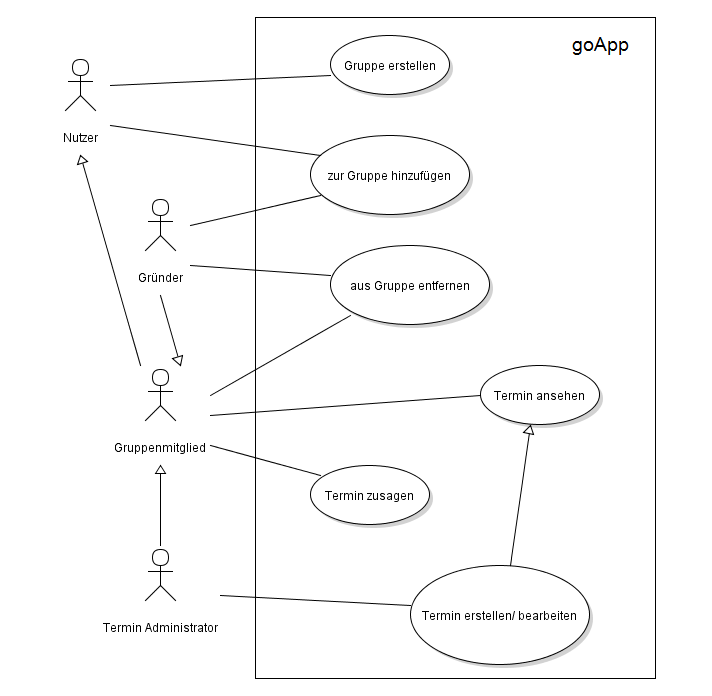
\includegraphics[width=\textwidth]{goApp_useCase}
	\end{figure}
	
	\newpage
	
	\subsection{Szenarien}
	%TODO: Stimmen Zeiten der Benachrichtigungen?
	\subsubsection{Szenario 1}
	Alice, Bob und Carol gehen oft gemeinsam in der Mensa essen. Zur besseren Koordination haben sie die App auf ihren Android-Smartphones installiert.
	Nun startet jeder bei sich die App und gibt, nachdem er sich über sein Google Account angemeldet hat, seinen Namen ein.
	Alice gründet nun eine neue Gruppe mit dem Namen ABC-Mensa. Danach geben Bob und Carol in das Suchfeld ABC-Mensa ein und klicken auf die entsprechende Gruppe.
	Es erscheint nun auf dem Display die Nachfrage ob sie der Gruppe beitreten wollen. Sobald sie dies bestätigt haben klickt Alice auf die Gruppe,
	sieht die Namen Bob und Carol als Bewerber, und fügt beide hinzu.
	Bob bekommt nun Hunger, klickt auf die Gruppe und erstellt einen neuen Termin mit dem Namen Mensa, dem entsprechenden Datum, der Uhrzeit 12:30 und dem Ort der Mensa.
	Kurze Zeit darauf schauen Alice und Carol auf ihr Smartphone, sehen den Termin und klicken beide auf \glqq{}Teilnehmen\grqq{}.
	Um 12:15 erscheint auf allen Smartphones die Benachrichtigung, dass in 15 Minuten der Termin ansteht.
	Alle gehen kurz daraufhin los und können in der App sowohl ihren als auch den mittleren Gruppenstandort sehen.
	Nachdem der Termin vorbei ist, wird er automatisch gelöscht.
	\newline
	\newline
	\begin{figure}[h]
	\centering
	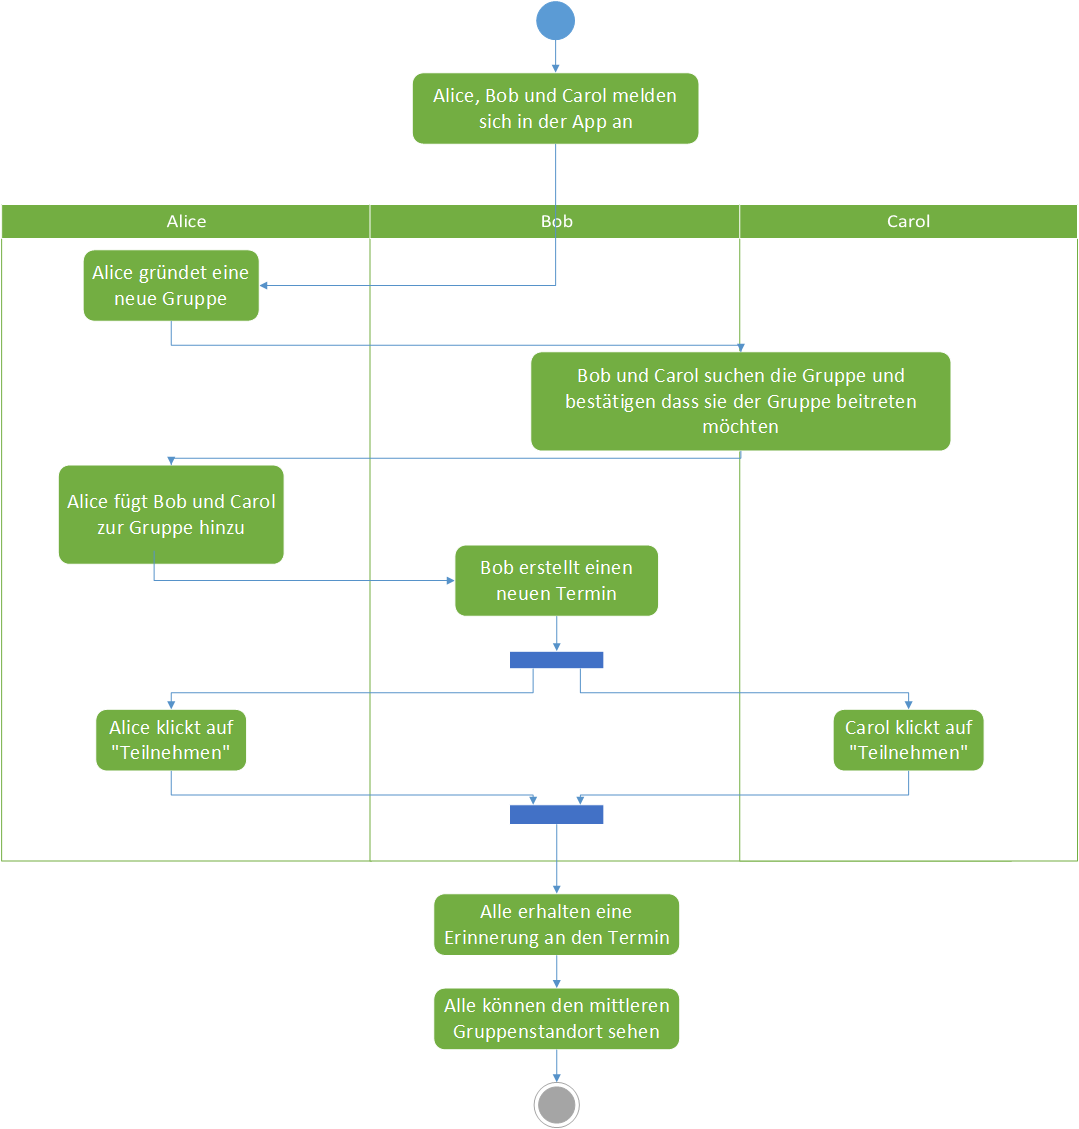
\includegraphics[width=\textwidth]{Szenario1}
	\end{figure}
	
	\newpage
	
	
	\subsubsection{Szenario 2}
	Die Personen Alice, Bob, Carol, Dave und Eve sind in einer gemeinsamen Gruppe.
	Alice will um 12:00 Uhr in die Mensa gehen. Daher erstellt Alice in der Gruppe einen neuen Termin \glqq{}Mensa 12:00\grqq{}.
	Alle anderen Gruppenmitglieder sehen den neuen Termin. Bob und Carol wollen auch um 12:00 in die Mensa gehen und klicken auf \glqq{}Teilnehmen\grqq{}.
	Dave und Eve müssen um 12:00 Uhr noch etwas erledigen und können deshalb erst später in die Mensa, sie klicken deshalb auf \glqq{}Nicht Teilnehmen\grqq{}.
	Da sie auf \glqq{}Nicht Teilnehmen\grqq{} geklickt haben, ist der Termin für sie nicht mehr sichtbar.
	Dave erstellt später einen neuen Termin \glqq{}Mensa 12:30\grqq{} in der Gruppe.
	Um 12:30 hat Eve auch Zeit und klickt auf \glqq{}Teilnehmen\grqq{}.
	Da Alice, Bob und Carol schon früher in die Mensa gehen klicken sie auf \glqq{}Nicht Teilnehmen\grqq{}.
	Um 11:45 werden Alice, Bob und Carol an ihren Termin erinnert und um 12:15 Dave und Eve.
	Der mittlere Gruppenstandort bezieht sich immer ausschließlich auf die Personen, die an dem Termin teilnehmen.
	So sieht Alice den mittleren Standort von sich, Bob und Carol.	
	\newline
	\newline
	\newline
	\begin{figure}[h]
		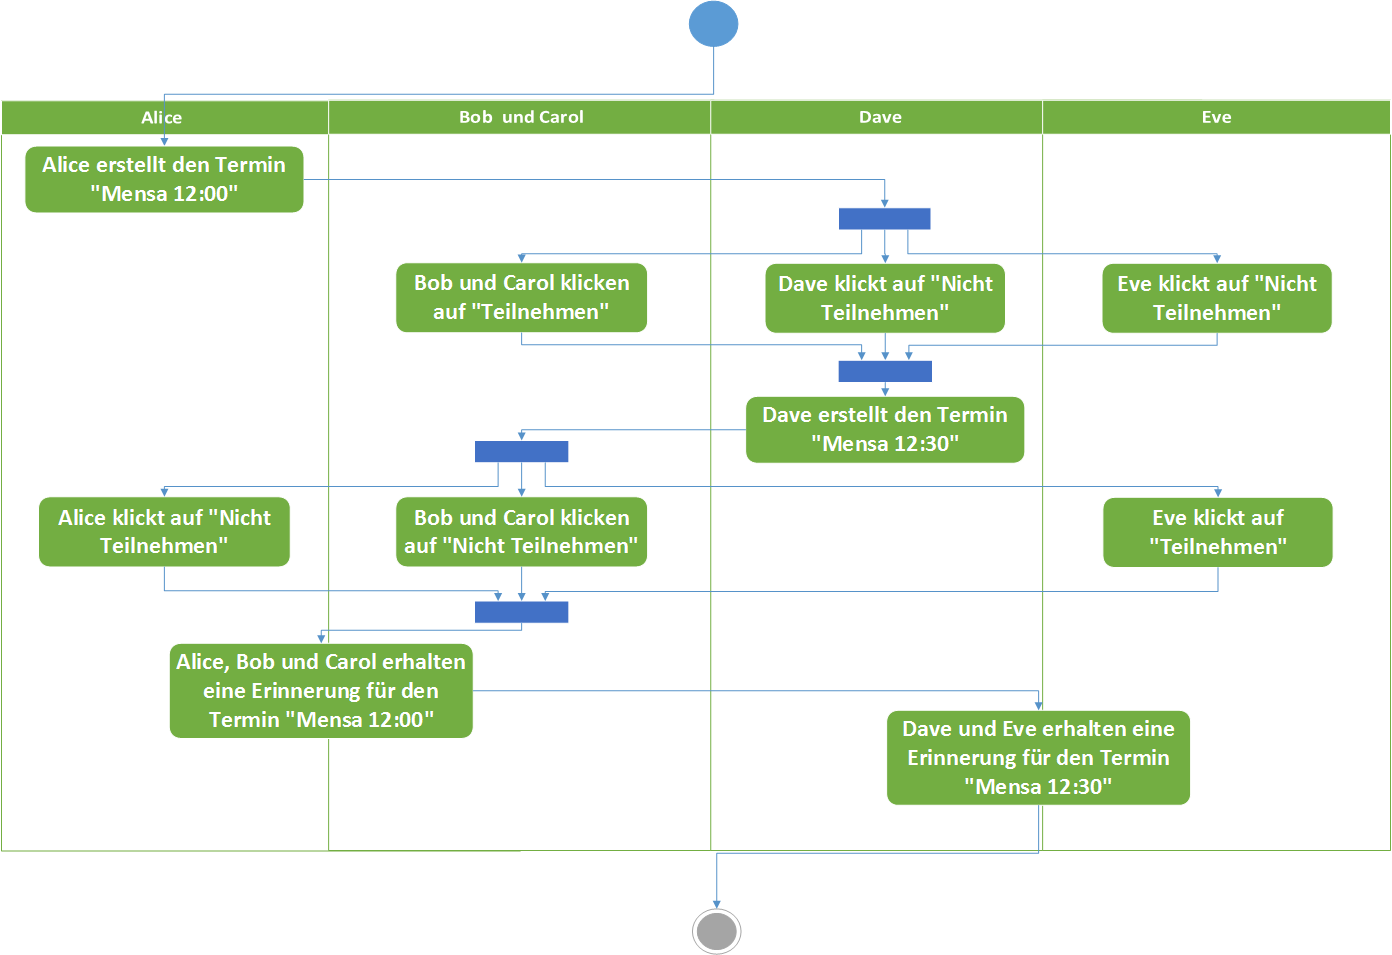
\includegraphics[width=\textwidth]{Szenario2}
	\end{figure}
	\newpage
	
	\subsubsection{Szenario 3}
	Es gibt die Personen Alice, Bob, Carol und Dave, welche alle bereits in der App registriert sind.
	Alice hat Geburtstag und erstellt deshalb eine neue Gruppe mit dem Namen \glqq{}Geburtstag Alice\grqq{}. Die anderen geben in das Suchfeld \glqq{}Geburtstag Alice\grqq{} ein und klicken auf die passende Gruppe.
	Jetzt erscheint die Nachfrage, ob sie der Gruppe beitreten wollen. Alice sieht nun, welche von ihren Gästen teilnehmen wollen und fügt diese hinzu. Dave möchte auch beitreten, aber Alice hat ihn nicht eingeladen und lehnt seine Anfrage ab.
	Sobald alle Gäste der Gruppe beigetreten sind, erstellt Alice einen neuen Termin mit dem Namen \glqq{}Feier\grqq{} und ihrem zu Hause als Ort, sowie dem Datum \glqq{}27.11.2016\grqq{} und die Uhrzeit \glqq{}21:00\grqq{}.
	Bob und Carol sehen den Termin und klicken auf \glqq{}Teilnehmen\grqq{}.
	Um 20:30 erscheint auf allen Smartphones die Benachrichtigung, dass in 30 Minuten der Termin ansteht. Alle gehen kurz daraufhin los und können in der App sowohl ihren als auch den mittleren Gruppenstandort sehen.
	Eine Stunde nachdem der Termin gestartet ist, wird er automatisch gelöscht.
	Am nächsten Tag verlässt Bob die Gruppe und Alice löscht daraufhin die Gruppe, da diese nicht mehr gebraucht wird.	
	\newline
	\newline
	\begin{figure}[h]
		\centering
		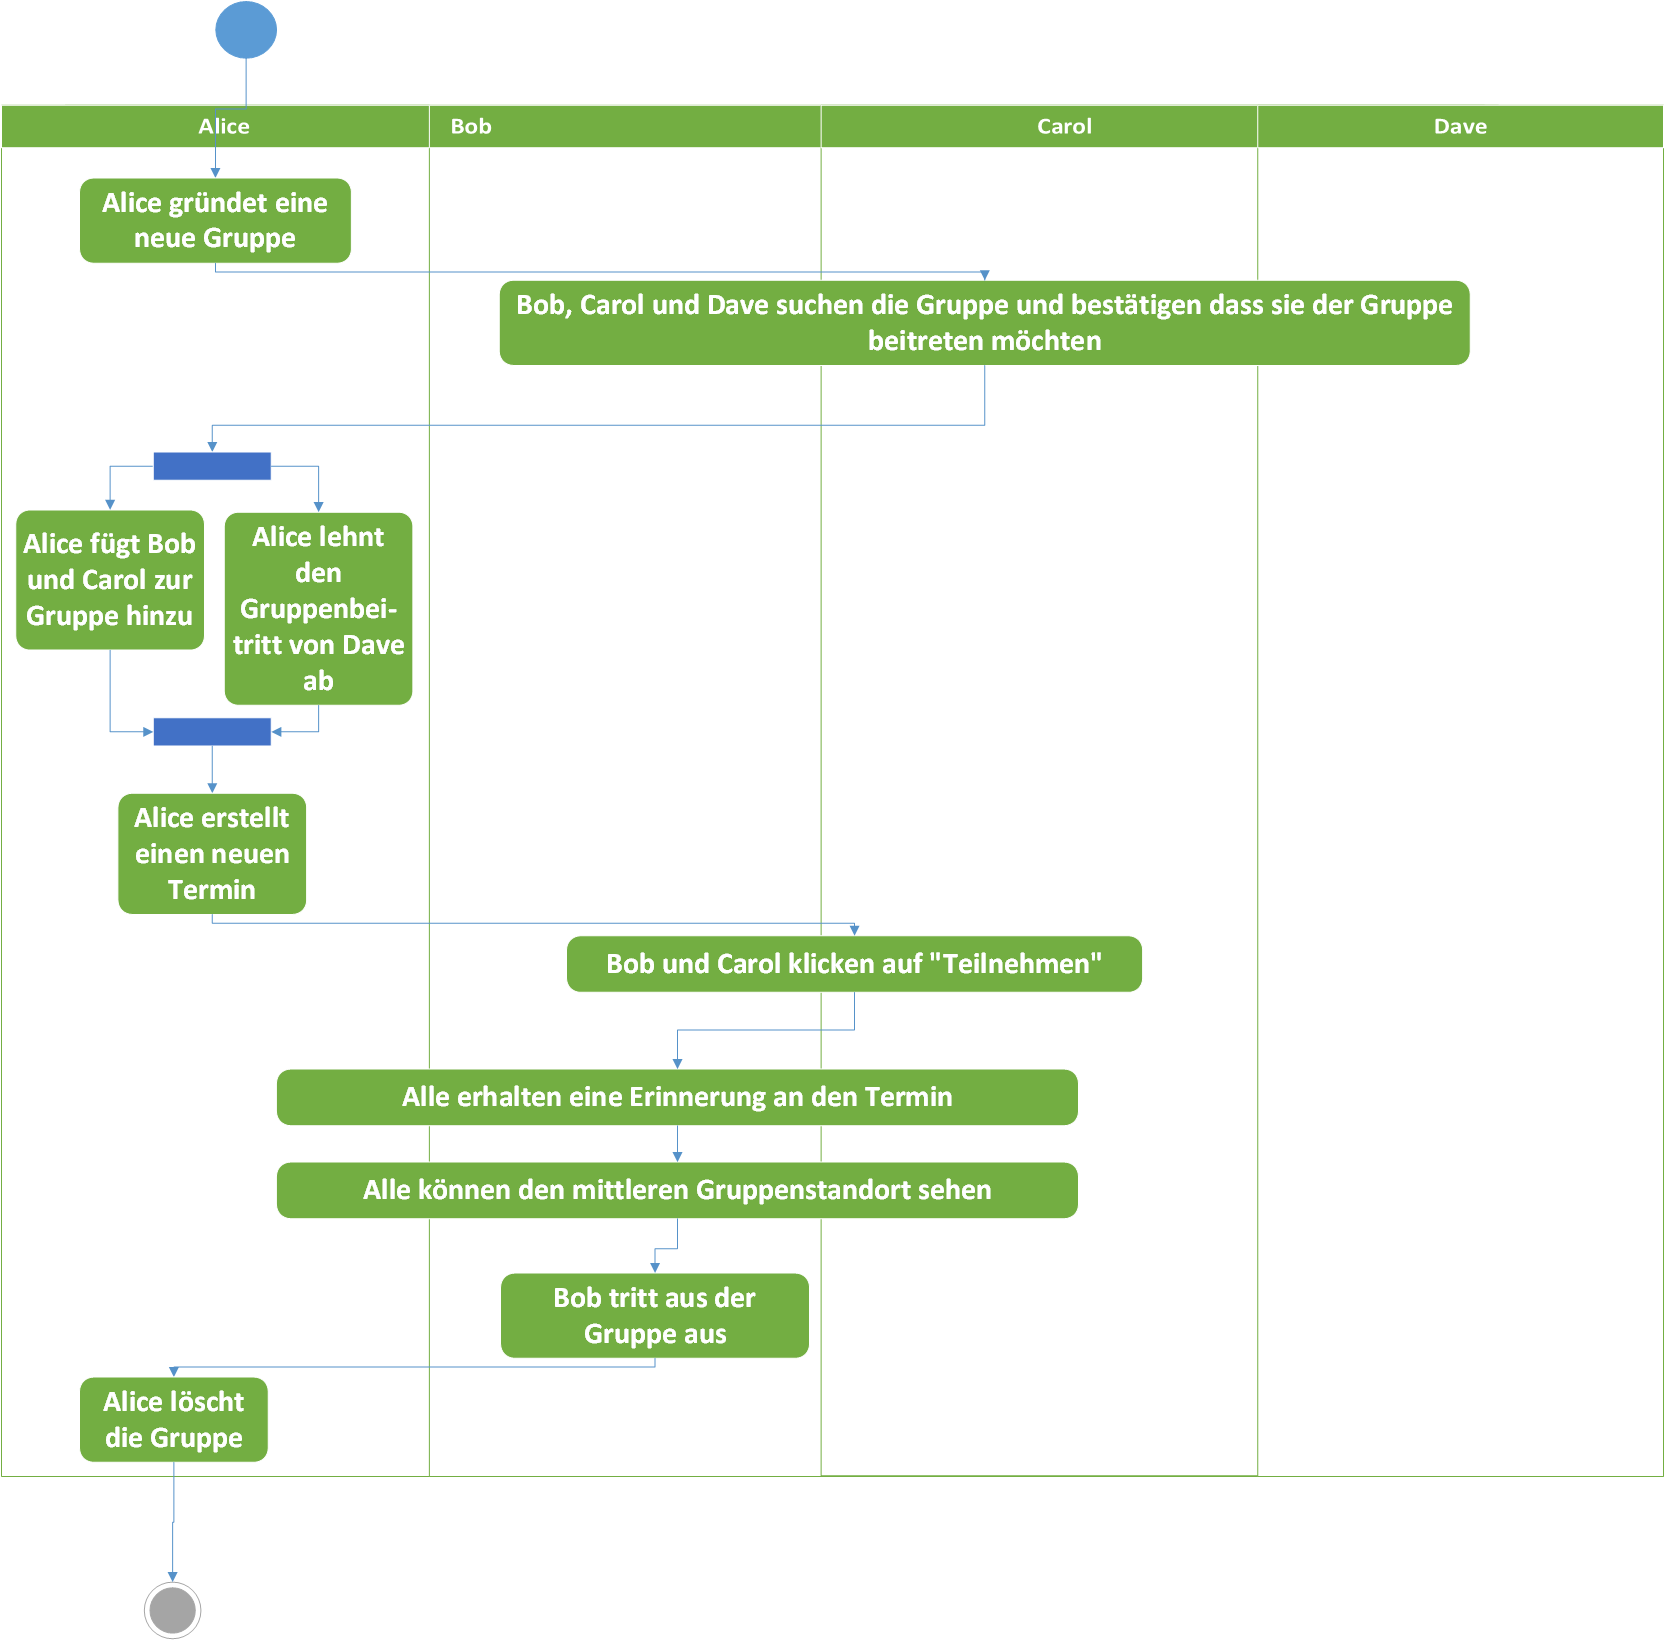
\includegraphics[width=0.8\textwidth]{Szenario3}
	\end{figure}
	\newpage
	
	\subsubsection{Szenario 4 (Wunschszenario)}
	Alice, Bob, Carol und Dave wollen sich am Abend im Restaurant \glqq{}Oxford\grqq{} in Karlsruhe zum Essen treffen. 
	Da sie alle die goApp installiert haben und einer gemeinsamen Gruppe angehören, erstellt Alice in der App 		einen Termin names \glqq{}Oxford\grqq{}, dem die drei anderen zusagen. Alice trifft Bob pünktlich um 8:00 Uhr im 		\glqq{}Oxford Pub\grqq{} kann jedoch Carol und Dave nicht finden, die in der App durch den \glqq{}Bin da\grqq{}-Button 		jedoch schon signalisiert haben vor Ort zu sein. Deshalb öffnet Alice die goApp und versucht über den Gruppenstandort 		mehr Information zu erhalten. Carol und Dave haben sich inzwischen in dem 200 Meter entfernten \glqq{}Oxford 			\grqq{} getroffen. Alice erkennt in der Karte der App durch die Clusteringanalyse neben dem Standort von ihr und 		Bob einen zweiten Standort, der zu Carol und Dave gehören muss. Sie bemerkt dadurch das Missverständnis zwischen 		\glqq{}Oxford Pub\grqq{} und \glqq{}Oxford Cafe\grqq{} sofort und macht sich mit Bob in Richtung \glqq{}Oxford 			Cafe\grqq{} auf.    \newline
	\newline
	\newline
	
	
	\begin{figure}[h]
		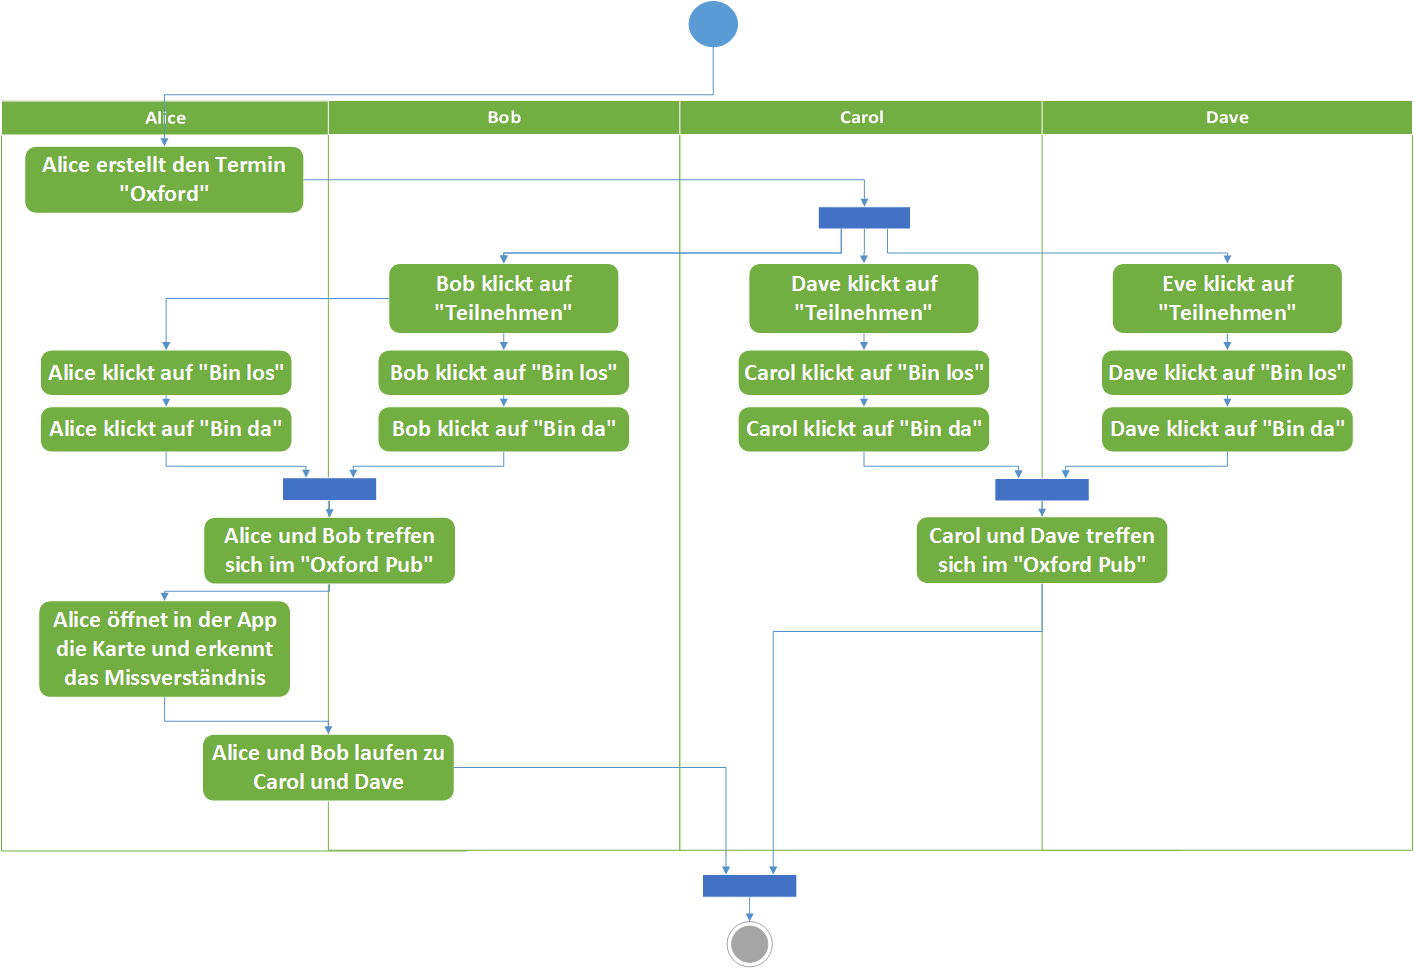
\includegraphics[width=\textwidth]{Szenario4}
	\end{figure}
	\newpage
	
	
	
	\newpage
	
	\subsection{GUI}
	\begin{figure}[h]
		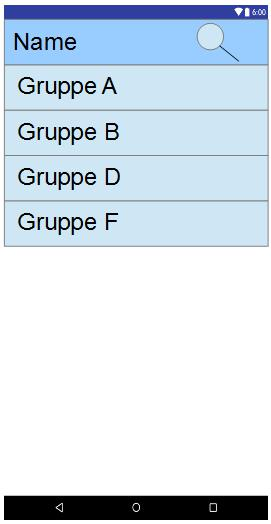
\includegraphics[width=.5\textwidth]{GUI_Start.jpg}
		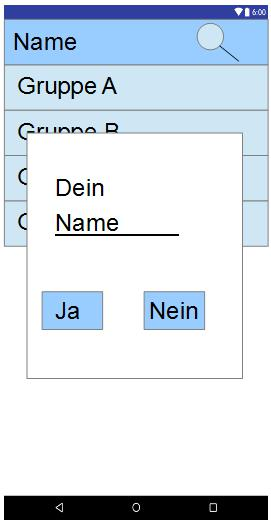
\includegraphics[width=.5\textwidth]{GUI_changeName.jpg}
		\caption{Die Startseite zeigt den Namen des Benutzers und bietet eine Übersicht über alle Gruppen in denen der Benutzer \gls{Mitglied} ist. Außerdem lässt sich hier der eigene Anzeigename ändern.}
	\end{figure}
	
	\newpage
	\begin{figure}[h]
		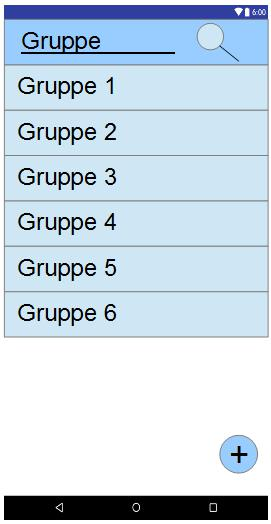
\includegraphics[width=.5\textwidth]{GUI_NeueGruppe.jpg}
		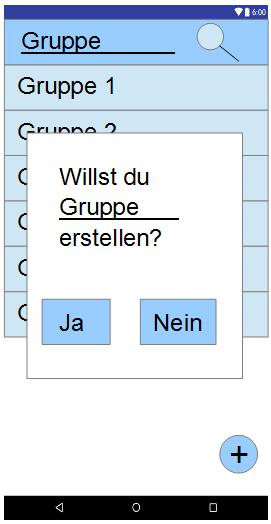
\includegraphics[width=.5\textwidth]{GUI_GruppeNeuBest.jpg}
		\caption{Die Gruppensuche zeigt dem Benutzer alle Gruppen an deren Name mit seiner Eingabe startet, zusätzlich kann der Benutzer hier eine neue Gruppe erstellen.}
	\end{figure}
	
	\newpage
	\begin{figure}[h]
		\centering
		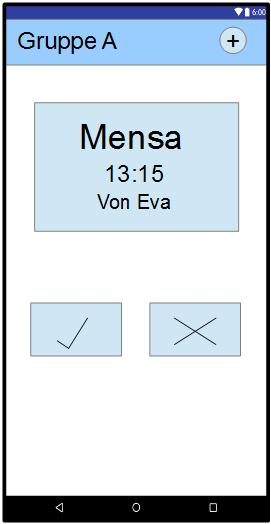
\includegraphics[width=.5\textwidth]{GUI_Gruppe.jpg}
		\caption{In einer Gruppe bekommt ein  \gls{Mitglied} die Termine der Gruppe angezeigt und kann bei diesen zu- oder absagen. Mit einem Wischen kann zwischen allen aktuellen Terminen gewechselt werden. Es kann ebenfalls ein eigener Termin erstellt und weitere Details sowohl über die Gruppe als auch die Termine abgerufen werden.}
	\end{figure}
	
	\newpage
	\begin{figure}[h]
		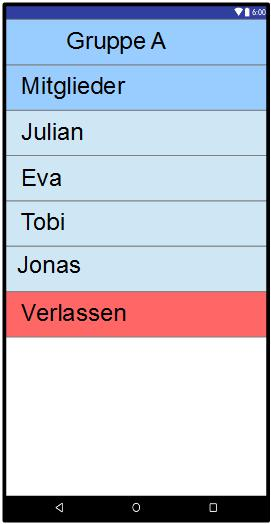
\includegraphics[width=.5\textwidth]{GUI_GruppeInfoNormal.jpg}
		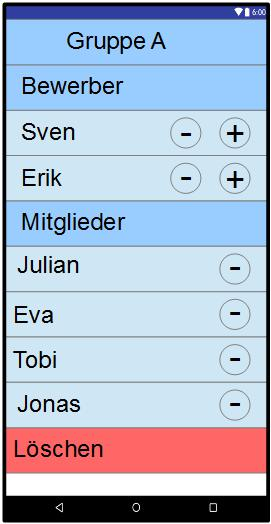
\includegraphics[width=.5\textwidth]{GUI_GruppeInfoGruender.jpg}
		\caption{In der Gruppeninformationsansicht sehen Mitglieder alle anderen Mitglieder der Gruppe und sie können die Gruppe verlassen. Der Gründer der Gruppe kann zusätzlich einzelne Mitglieder aus der Gruppe entfernen und Beitrittsanfragen bearbeiten, anstatt die Gruppe zu verlassen kann er die Gruppe löschen.}
	\end{figure}
	
	\newpage
	\begin{figure}[h]
		\centering
		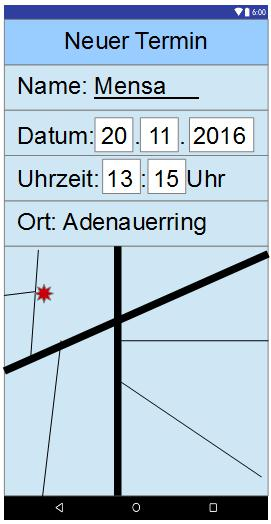
\includegraphics[width=.5\textwidth]{GUI_NeuerTermin.jpg}
		\caption{Damit ein \gls{Mitglied} einen neuen Termin erstellen kann, muss es dem Termin einen Namen geben und ihn mit Datum, Uhrzeit und einem Ort versehen.}
	\end{figure}
	
	\newpage
	\begin{figure}[h]
		\centering
		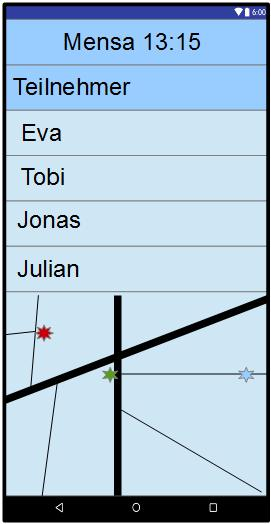
\includegraphics[width=.5\textwidth]{GUI_Termin.jpg}
		\caption{In der Terminansicht erhält ein \gls{Mitglied} alle Informationen über einen Termin. Darunter werden eine Teilnehmerliste und eine Karte, die den Treffpunkt sowie den eigenen Standort zeigt, angezeigt. Sollte der Termin kurz bevorstehen, ist zusätzlich der Gruppenmittelpunkt zu sehen.}
	\end{figure}
	
	
\newpage
	


\appendix
%\bibliographystyle{plainnat}
%\bibliography{bibtex}
\printindex
\glsaddall
\printglossaries
	
\end{document}
